% This is samplepaper.tex, a sample chapter demonstrating the
% LLNCS macro package for Springer Computer Science proceedings;
% Version 2.21 of 2022/01/12
%
\documentclass[runningheads]{llncs}
%
\usepackage[T1]{fontenc}
% T1 fonts will be used to generate the final print and online PDFs,
% so please use T1 fonts in your manuscript whenever possible.
% Other font encondings may result in incorrect characters.
%
\usepackage{graphicx}
\usepackage{amsmath}
\usepackage{amssymb}
\usepackage{subcaption}
\usepackage{multirow}
\usepackage{booktabs}




\setlength{\textfloatsep}{5pt} %Table up
\setlength{\floatsep}{5pt}  %Table up
\setlength{\intextsep}{5pt} %Table up
\usepackage{placeins}  % Float boundary control
\usepackage{float}      % Fixed float option

% Used for displaying a sample figure. If possible, figure files should
% be included in EPS format.
%
% If you use the hyperref package, please uncomment the following two lines
% to display URLs in blue roman font according to Springer's eBook style:
\usepackage{color}
\usepackage{url}
\renewcommand\UrlFont{\color{blue}\rmfamily}
\urlstyle{rm}
%\renewcommand\UrlFont{\color{blue}\rmfamily}
%\urlstyle{rm}
%
\begin{document}
%
\title{Cross-Robot Knowledge Transfer for Quadrupedal Control via In-Context Reinforcement Learning}
%
\titlerunning{Cross-Robot Knowledge Transfer for Quadrupedal Control}
% If the paper title is too long for the running head, you can set
% an abbreviated paper title here
%

\author{Naoaki Ishii\inst{1}%\orcidID{0000-0002-3430-8180} 
\and
Hiroshi Kera\inst{1, 2}%\orcidID{0000-0002-9830-0436}
\and
Kazuhiko Kawamoto\inst{1}%\orcidID{0000-0003-3701-1961}
}

%
\authorrunning{Ishii et al.}
% First names are abbreviated in the running head.
% If there are more than two authors, 'et al.' is used.
%


\institute{Chiba University, Chiba 263-8522, Japan \\
\and
National Institute of Informatics, Tokyo 101-8430, Japan
\\
\email{naoaki.ishii@chiba-u.jp,kera@chiba-u.jp,kawa@faculty.chiba-u.jp}}


%
\maketitle              % typeset the header of the contribution
%
\begin{abstract}
Deep reinforcement learning policies for quadrupedal locomotion often depend on the dynamics of the training robot. 
As a result, transferring a policy to a different robot can require costly retraining.
Existing methods improve generalization by increasing the diversity of robot dynamics during training, but this requires additional data and computation.
This study investigates whether a pretrained policy can be adapted to a robot excluded from training by updating only its action mapping.
Algorithm distillation trains a causal Transformer on continuous-noise-distillation data from three robots. 
Decoder-only adaptation then keeps the history encoder fixed and updates only the decoder using 10\% of the available target-robot data.
Leave-one-robot-out experiments in the Genesis simulator with Go1, Go2, A1, and Mini Cheetah show that decoder-only adaptation yields higher average episode returns than zero-shot transfer for all four robots.
These results indicate that a history representation learned across multiple robots can support cross-robot adaptation through updates limited to the output mapping.


\keywords{Reinforcement Learning \and Algorithm Distillation \and Quadrupedal Locomotion \and Transfer Learning}
\end{abstract}


\section{Introduction}
\label{sec:introduction}

Deep reinforcement learning (DRL) has achieved strong performance in robot control~\cite{annurev:/content/journals/10.1146/annurev-control-030323-022510}. However, locomotion policies often depend strongly on the dynamics of the robot used during training. 
Differences in mass, inertia, morphology, and actuation can substantially degrade policy performance when the policy is transferred to another robot~\cite{9308468,NEURIPS2018_b8cfbf77}.
Training a separate policy for every robot requires
substantial interaction and computation.
Therefore, transferring locomotion knowledge across robots remains an important challenge.


Existing approaches mainly address this challenge in two ways.
The first approach broadens the training distribution through domain randomization or multi-task learning~\cite{8202133,pmlr-v100-yu20a}.
These methods improve robustness but require training over a sufficiently diverse range of environments and dynamics.
The second approach adapts policy behavior from interaction histories.
In-context reinforcement learning methods condition their actions on previous observations, actions, and rewards~\cite{duan2016rl2fastreinforcementlearning,NEURIPS2021_7f489f64}.
Algorithm distillation further learns an implicit policy-improvement process from such histories~\cite{laskin2022incontextreinforcementlearningalgorithm,zisman2024emergenceincontextreinforcementlearning}, and Vintix applies this framework to robotic control~\cite{polubarov2025vintixactionmodelincontext}.
However, the resulting policy still depends on the robot embodiments represented in the training data. Interaction histories alone may not sufficiently compensate for the dynamics of a previously unseen robot.


This work examines which part of an algorithm-distilled policy should be adapted to a new robot. 
We hypothesize that the history-dependent features required for quadrupedal locomotion contain information that is transferable across robots, whereas the mapping from these features to joint commands is more robot-specific. 
Based on this hypothesis, we separate the policy into a shared encoder and an action decoder. 
The encoder extracts a latent representation from the interaction history and the current observation, and the decoder maps this representation to control actions. 
During pre-training, both components are jointly trained on data from multiple robots. 
During adaptation, the encoder remains fixed, and only the decoder is fine-tuned using data from the unseen robot. 
This design retains the pretrained history representation while adapting the output mapping to the target robot.


%In this study, we propose an adaptation method that decomposes an algorithm distillation model into two components: one that extracts internal representations useful for locomotion and another that maps these representations to robot-specific control signals. We assume that the representations required for locomotion are shared across different robots, whereas robot-specific differences are mainly reflected in the output mapping to control signals. Based on this assumption, we freeze the shared internal representations and fine-tune only the decoder responsible for the output mapping, enabling adaptation to unseen robots while preserving previously acquired locomotion skills. This approach aims to achieve stable locomotion on unseen robots with minimal additional training.

We evaluate the proposed method in the Genesis simulator using four
quadruped robots: Go1, Go2, and A1 developed by Unitree
Robotics~\cite{unitree_updated}, and Mini Cheetah developed by the
Massachusetts Institute of Technology~\cite{8793865}.
Figure~\ref{fig:robot_sim_views} shows the four robots.
We conduct leave-one-robot-out experiments in which the model is pretrained on three robots and adapted to the remaining robot.
For adaptation, we use 10\% of the target-robot dataset generated from its PPO expert and fine-tune the decoder for two epochs.
Decoder-only adaptation improves the average
cumulative reward for all four held-out robots and reaches 85.7--99.6\% of the reward obtained by the corresponding expert policies.

The main contributions of this work are as follows:
\begin{itemize}
\item We introduce a decoder-only adaptation method for transferring an algorithm-distilled locomotion policy to an unseen robot while keeping its history encoder fixed.
\item We examine the hypothesis that a history-dependent locomotion representation can be shared across quadruped robots, while the action mapping requires robot-specific adaptation. Our results are consistent with this hypothesis, but they do not isolate the contribution of the encoder.
\item We evaluate the method in a leave-one-robot-out setting with four simulated quadruped robots. The adapted policies reach 85.7--99.6\% of the corresponding expert-policy rewards using 10\% of the available target-robot data.
\end{itemize}

\begin{figure}[t]
  \centering

  \begin{subfigure}{0.24\linewidth}
    \centering
    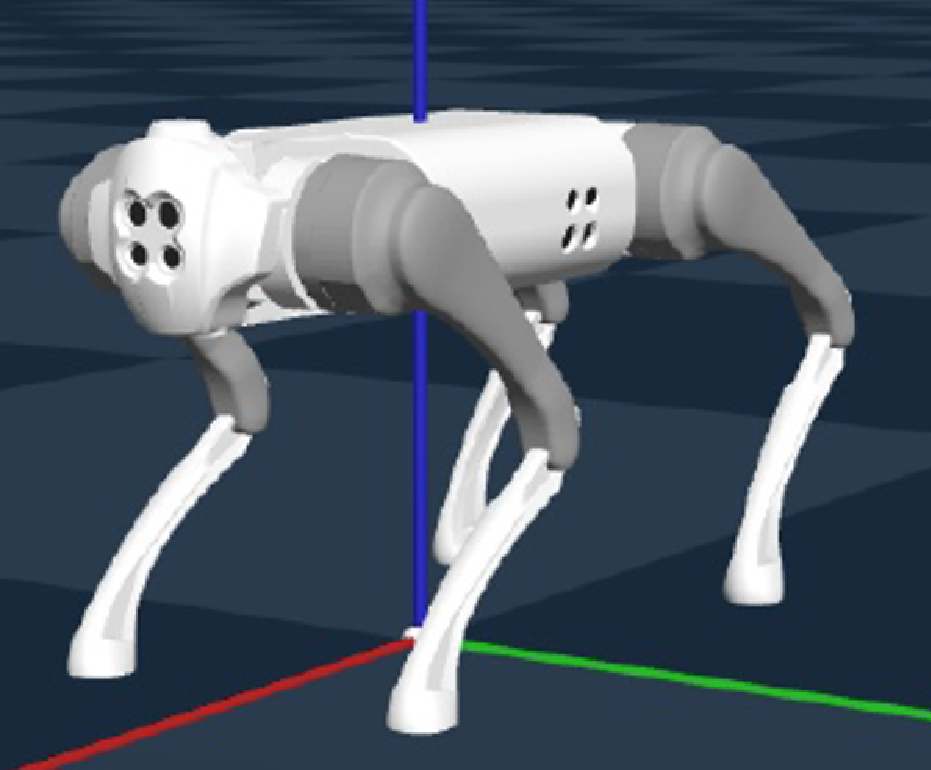
\includegraphics[width=\linewidth]{figs/go1_target_height_diagonal.pdf}
    \caption{Go1}
  \end{subfigure}
  \hfill
  \begin{subfigure}{0.24\linewidth}
    \centering
    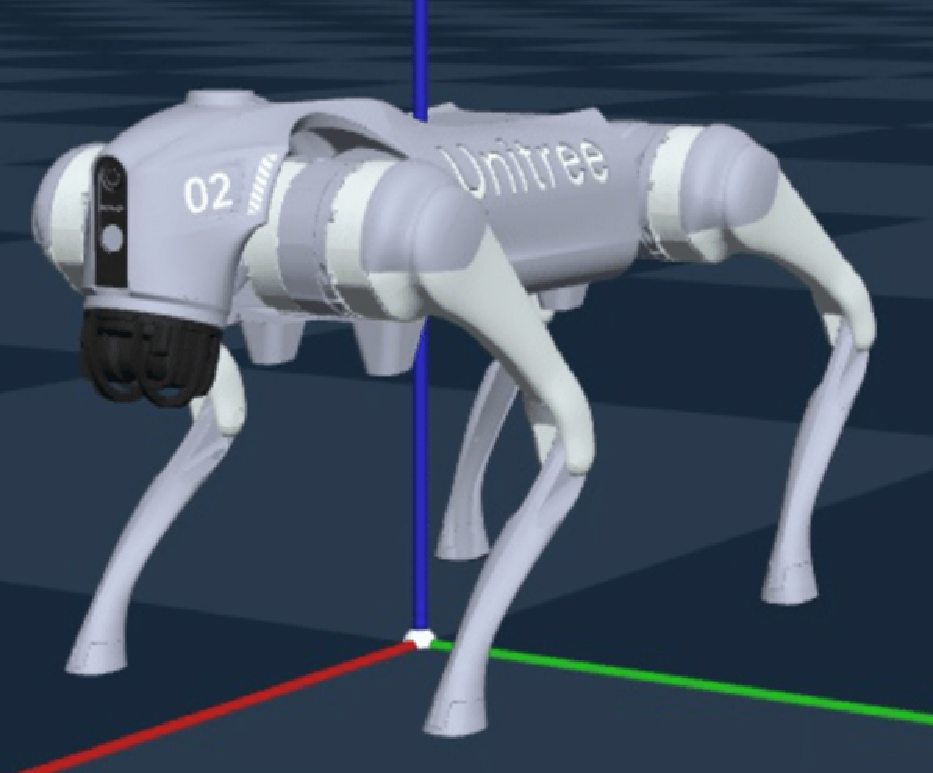
\includegraphics[width=\linewidth]{figs/go2_target_height_diagonal.pdf}
    \caption{Go2}
  \end{subfigure}
  \hfill
  \begin{subfigure}{0.24\linewidth}
    \centering
    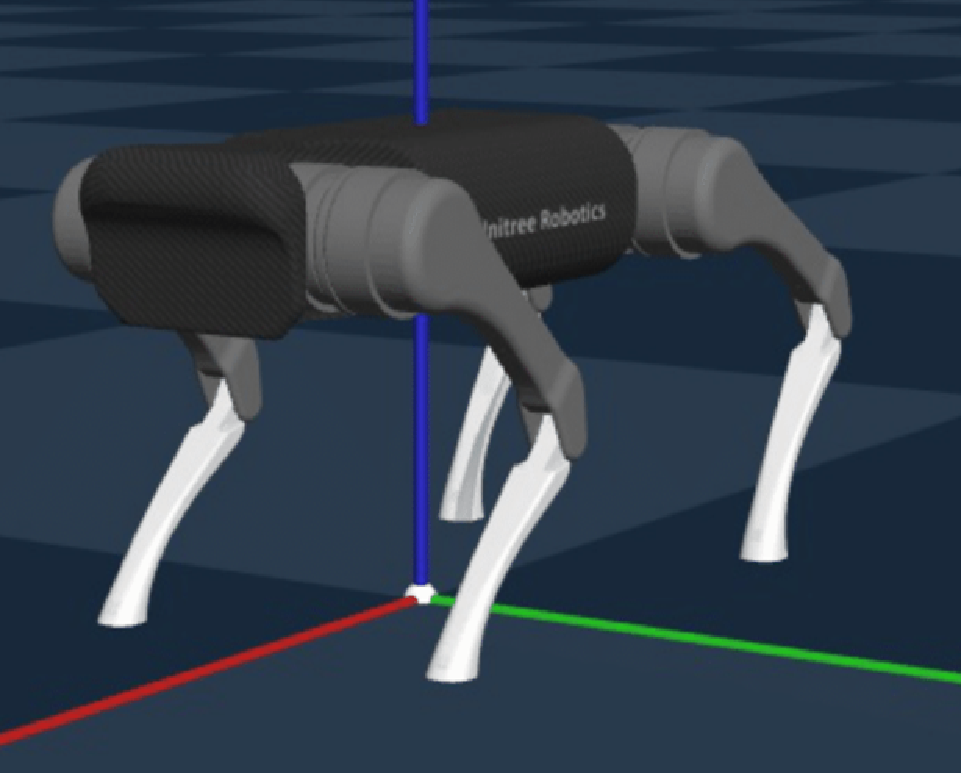
\includegraphics[width=\linewidth]{figs/a1_target_height_diagonal.pdf}
    \caption{A1}
  \end{subfigure}
  \hfill
  \begin{subfigure}{0.24\linewidth}
    \centering
    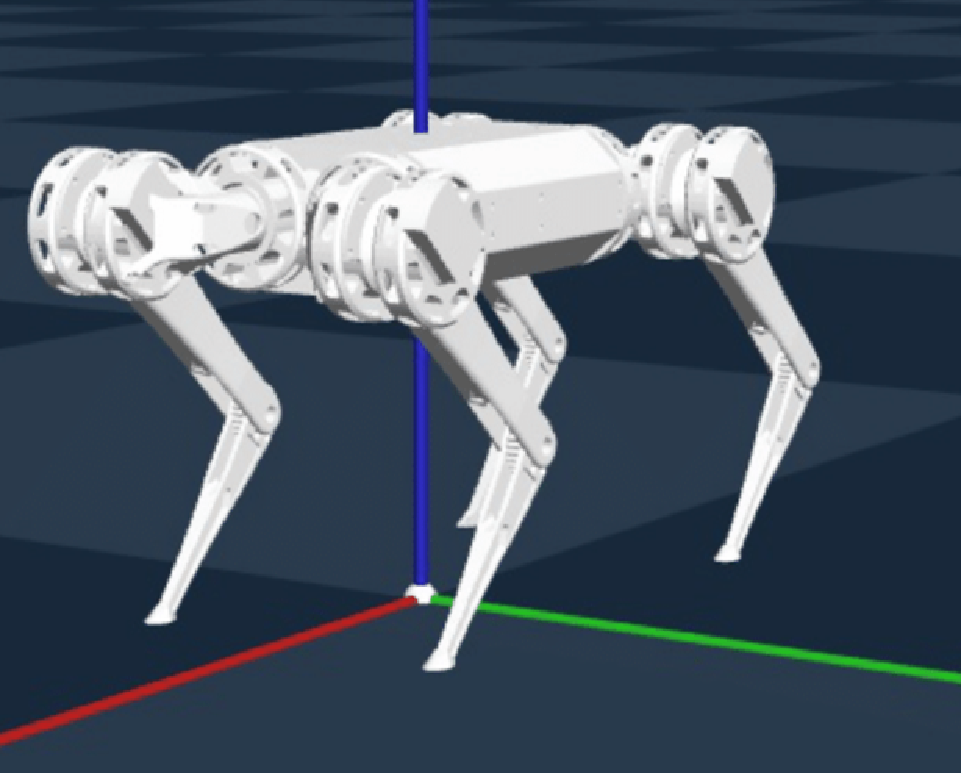
\includegraphics[width=\linewidth]{figs/minicheetah_target_height_diagonal.pdf}
    \caption{Mini Cheetah}
  \end{subfigure}

  \caption{Overview of the quadrupedal robots used in the experiments.}
  \label{fig:robot_sim_views}
\end{figure}

\section{Related Work}
\label{sec:related_work}

\subsection{Cross-Robot Generalization and Adaptation}
\label{sec:cross-robot}

%Policies learned by deep reinforcement learning tend to overfit to the environmental conditions and dynamics encountered during training. As a result, their performance often degrades when the robot morphology or physical parameters differ from those used during training~\cite{9308468}. To address this issue, domain randomization, which randomizes physical parameters during training~\cite{8202133,8460528}, and multi-task learning, which trains a single model across multiple tasks~\cite{pmlr-v100-yu20a}, have been proposed. Although these methods improve the robustness of learned policies, increasing the diversity of training conditions also increases the training cost.

Locomotion policies often degrade when they are transferred to robots with different morphology or dynamics~\cite{9308468}. Domain randomization improves robustness by varying physical parameters during training~\cite{8202133,8460528}. GenLoco extends this approach by randomizing robot morphology and dynamics to learn controllers that generalize across quadruped robots~\cite{pmlr-v205-feng23a}. However, these methods require the training distribution to cover the target robot sufficiently well.

Other methods explicitly model differences among robot embodiments. 
Hardware-conditioned policies~\cite{NEURIPS2018_b8cfbf77}, MetaMorph~\cite{gupta2022metamorph}, Universal Morphology Control~\cite{pmlr-v202-xiong23a}, and One Policy to Run Them All~\cite{pmlr-v270-bohlinger25a} learn shared policies conditioned on robot morphology or structure. REvolveR instead transfers a policy by gradually transforming a source robot into a target robot~\cite{pmlr-v162-liu22p}. These studies mainly seek zero-shot generalization or train a universal policy across embodiments. In contrast, our method adapts an algorithm-distilled policy to a held-out robot by updating only its action decoder.

%\subsection{Offline Reinforcement Learning}
%\label{sec:offline_rl}

%Offline reinforcement learning (offline RL) is a framework that learns policies solely from pre-collected datasets and achieves high sample efficiency through data reuse~\cite{levine2020offlinereinforcementlearningtutorial}. Representative methods include Batch-Constrained Q-learning (BCQ)~\cite{pmlr-v97-fujimoto19a} and Conservative Q-Learning (CQL)~\cite{NEURIPS2020_0d2b2061}, which achieve stable learning by suppressing out-of-distribution actions and preventing overestimation of value functions, respectively. However, because policies learned by offline RL are fixed to the distribution of the training data, adapting to environmental changes during deployment remains difficult.

\subsection{In-Context Reinforcement Learning and Algorithm Distillation}
\label{sec:incontext_rl}

In-context reinforcement learning (in-context RL) adapts policy behavior from interaction histories without parameter updates.
RL$^2$ uses a recurrent state to summarize previous observations, actions, and rewards~\cite{duan2016rl2fastreinforcementlearning}.
Related sequence-modeling approaches, such as Decision Transformer, formulate offline reinforcement learning as return-conditioned sequence modeling~\cite{NEURIPS2021_7f489f64}.

Algorithm Distillation trains a causal sequence model on complete reinforcement-learning histories and learns to reproduce policy improvement within its context~\cite{laskin2022incontextreinforcementlearningalgorithm}. 
Noise Distillation generates such histories by gradually reducing noise added to expert actions~\cite{zisman2024emergenceincontextreinforcementlearning}, and Vintix extends Algorithm Distillation to multiple tasks and robotic control domains~\cite{polubarov2025vintixactionmodelincontext}.

Unlike these methods, our approach addresses a target robot whose physical characteristics are absent from the pre-training data. We keep the pretrained history encoder fixed and fine-tune only the action decoder. This setting examines whether the history representation can be reused across robots while the output mapping is adapted to the target robot.

\section{Proposed Method}
\label{sec:proposed_method}

We propose decoder-only adaptation of an algorithm-distilled locomotion policy to a robot excluded from pre-training. 
We hypothesize that history-dependent locomotion features learned across multiple robots can be reused, whereas the mapping from these features to control actions requires robot-specific adaptation. 
Based on this hypothesis, the proposed method separates the policy into a shared history encoder and an action decoder. 
During adaptation, the encoder remains fixed, and only the decoder is fine-tuned. 
Our implementation follows the Vintix framework~\cite{polubarov2025vintixactionmodelincontext}. 
Figure~\ref{fig:vintix_architecture} illustrates the overall procedure.

%a transfer learning method that acquires locomotion skills shared across multiple robots through algorithm distillation and enables adaptation to unseen robots using only a small amount of data. The proposed method is based on a decoupled architecture consisting of two key ideas: (1) extracting a control structure shared among different robots into a latent space, and (2) updating only the output mapping during the adaptation stage. Vintix~\cite{polubarov2025vintixactionmodelincontext} is employed as the algorithm distillation framework. An overview of the proposed learning framework is shown in Fig.~\ref{fig:vintix_architecture}.

\begin{figure}[tbp]
  \centering
  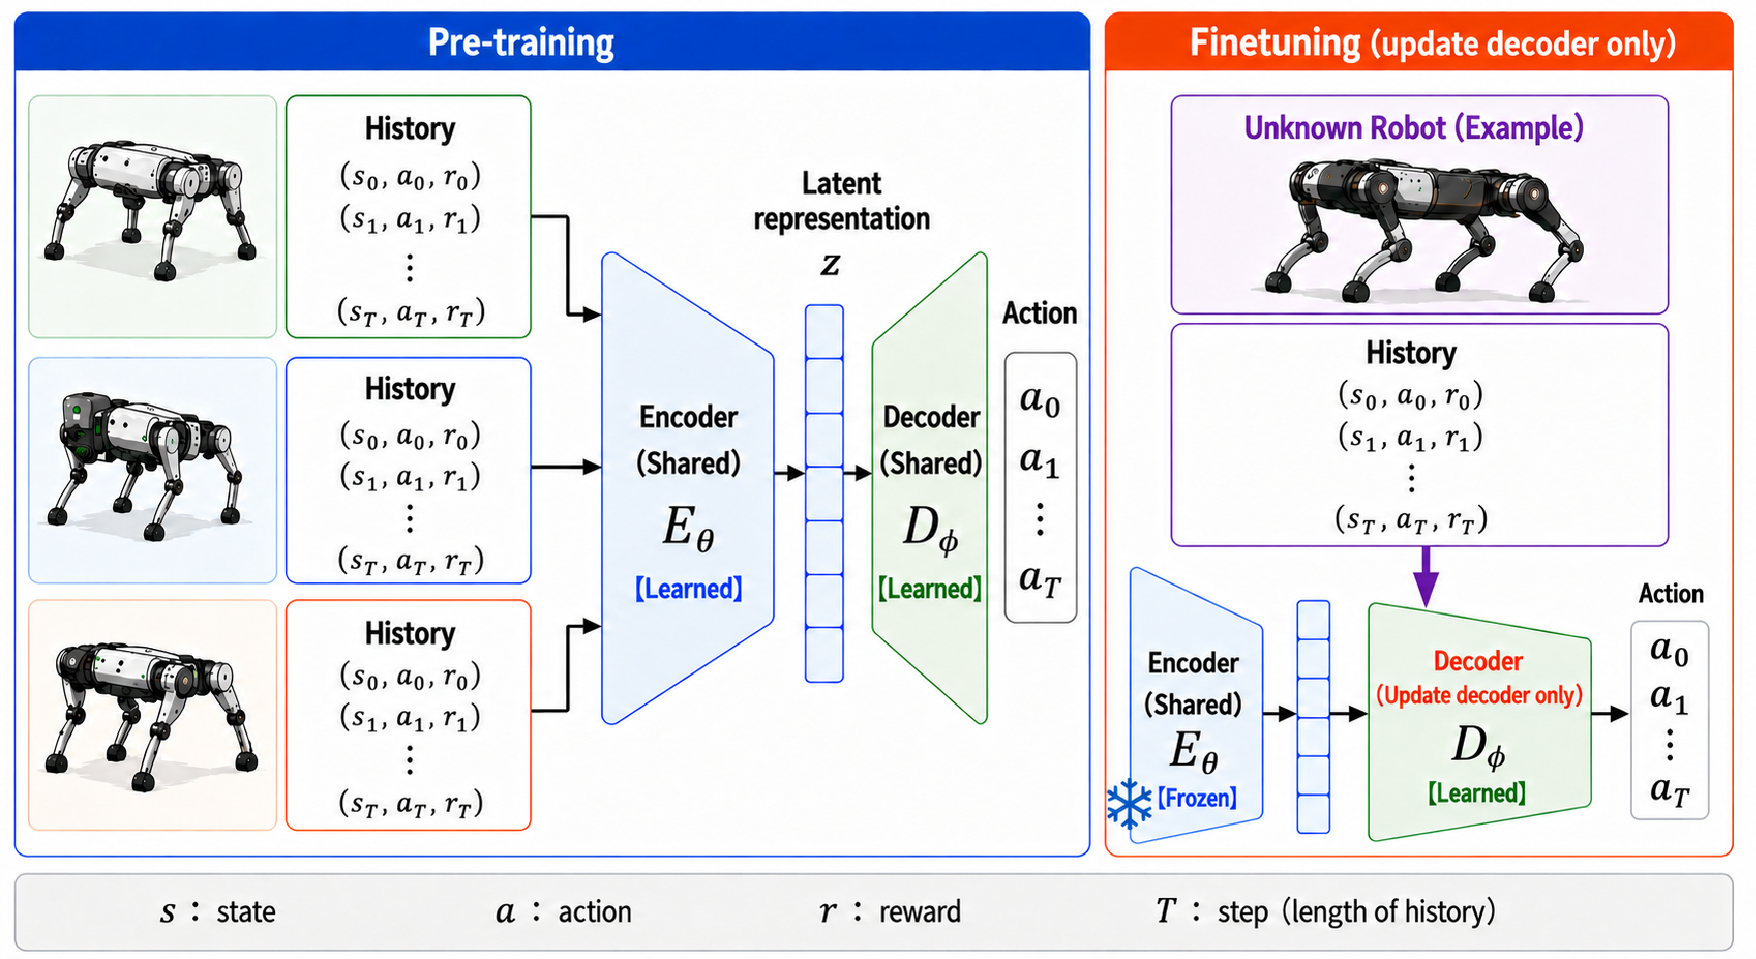
\includegraphics[width=\linewidth]{figs/vintix_architecture.pdf}
  \caption{
  Overview of the proposed method. Pre-training jointly optimizes the history encoder $E_\theta$ and action decoder $D_\phi$ using continuous-noise-distillation data from multiple robots. For a robot excluded from pre-training, the encoder is fixed, and only the decoder is fine-tuned using target-robot demonstrations.
  }
  \label{fig:vintix_architecture}
\end{figure}

\subsection{Problem Formulation: Cross-Robot Transfer Learning}

Let $\mathcal{N}=\{1,\ldots,N\}$ denote a set of robots that perform the same quadrupedal locomotion task. 
We divide this set into the pre-training robots $\mathcal{N}_{\mathrm{train}}\subset\mathcal{N}$ and a held-out target robot
$n_{\mathrm{tar}}\in\mathcal{N}\setminus\mathcal{N}_{\mathrm{train}}$.

Each robot induces a partially observable control process
\begin{equation}
M^{(n)}
=
\left(
\mathcal{S}^{(n)},
\mathcal{A},
P^{(n)},
r,
\mathcal{O},
\Omega^{(n)},
\gamma
\right),
\label{eq:robot_pomdp}
\end{equation}
where $\mathcal{S}^{(n)}$ is the state space, $\mathcal{A}$ is the action space, $P^{(n)}$ is the transition model, $r$ is the reward function, $\mathcal{O}$ is the observation space, $\Omega^{(n)}$ is the observation model, and $\gamma$ is the discount factor.
All robots share observation and action spaces of the same dimensionality and use the same reward definition. 
Their transition and observation models differ because of their physical characteristics.


The objective is to use data from the pre-training robots to obtain a policy for the held-out robot that achieves a high expected return:
\begin{equation}
J^{(n_{\mathrm{tar}})}=
\mathbb{E}\left[\sum_{t\ge0}\gamma^t r_t^{(n_{\mathrm{tar}})}\right].
\end{equation}
Rather than updating the entire policy for the target robot,
the proposed method updates only its action decoder.

\subsection{Shared History Encoder and Action Decoder}

Let $h_{t-1}^{(n)}$ denote the interaction history of robot $n$ before time step $t$:
\begin{equation}
h_{t-1}^{(n)}
=
\left(
(o_0^{(n)},a_0^{(n)},r_0^{(n)}),
\ldots,
(o_{t-1}^{(n)},a_{t-1}^{(n)},r_{t-1}^{(n)})
\right).
\label{eq:history_def}
\end{equation}
The shared encoder $E_\theta$ maps the interaction history and current observation to a latent representation:
\begin{equation}
z_t^{(n)}=E_\theta
(h_{t-1}^{(n)},o_t^{(n)}),
\quad
z_t^{(n)}\in\mathcal{Z}\subset\mathbb{R}^{d_z}.
\label{eq:latent_representation}
\end{equation}
The decoder $D_\phi$ maps the latent representation to an action:
\begin{equation}
\hat{a}_t^{(n)}=D_\phi(z_t^{(n)}).
\label{eq:decoder_mapping}
\end{equation}
The resulting history-conditioned policy is
\begin{equation}
\label{eq:policy_comp}
\pi_{\theta,\phi}(h_{t-1}^{(n)},o_t^{(n)})
=D_\phi(E_\theta(h_{t-1}^{(n)},o_t^{(n)})).
\end{equation}

The encoder is shared across the pre-training robots and is intended to capture transferable history-dependent locomotion features.
The decoder maps these features to robot control actions.
Both components are jointly optimized during pre-training.
For the held-out robot, the encoder remains fixed, and only the decoder is adapted.



\subsection{Pre-training with Continuous Noise Distillation}

Algorithm Distillation requires histories that represent policy improvement.
Recording complete reinforcement-learning processes is expensive because early exploration is inefficient and the policy distribution changes during training.
We therefore use continuous noise distillation to generate synthetic improvement histories efficiently~\cite{zisman2024emergenceincontextreinforcementlearning,polubarov2025vintixactionmodelincontext}.

For robot $n$, the executed action combines an expert action with uniformly sampled noise:
\begin{equation}
a_t^{(n)}=(1-\epsilon_t)
\pi_n^{\mathrm{expert}}(o_t^{(n)})
+
\epsilon_t u_t,
\end{equation}
where $u_t$ is sampled uniformly from the normalized action range.

The noise coefficient $\epsilon_t=\epsilon(n_s)$ decreases with the step index $n_s$: 
\begin{equation}
\epsilon(n_s)=
\begin{cases}
\sqrt[p]{1-\left(\dfrac{n_s}{(1-f)N_s}\right)^p}
& n_s\le(1-f)N_s \\
0 & \text{otherwise},
\end{cases}
\end{equation}
where $N_s$ is the number of steps in the generated sequence. 
The parameter $f\in[0,1)$ specifies the final proportion of the sequence without action noise, and $p>0$ controls the decay shape.
As $\epsilon(n_s)$ decreases, the generated behavior changes from noisy actions to expert-like actions.
The resulting sequence serves as a synthetic policy-improvement history.


Let $\mathcal{D}^{(n)}$ denote the dataset generated for pre-training robot $n$.
The shared encoder and decoder are optimized using the mean squared error:
\begin{equation}
\left(
\bar{\theta},
\bar{\phi}
\right)
=
\arg\min_{\theta,\phi}
\frac{1}
{\left|\mathcal{N}_{\mathrm{train}}\right|}
\sum_{n\in\mathcal{N}_{\mathrm{train}}}
\mathbb{E}_{
\left(h_{t-1},o_t,a_t\right)
\sim
\mathcal{D}^{(n)}
}
\left[
\left\|
a_t
-
D_\phi
\left(
E_\theta
\left(
h_{t-1},
o_t
\right)
\right)
\right\|_2^2
\right].
\label{eq:pretrain_obj}
\end{equation}

The model consists of an input embedding MLP, a causal Transformer~\cite{NIPS2017_3f5ee243}, and a decoder MLP. 
The input module embeds the interaction history and current observation.
The causal Transformer produces the latent representation $z_t\in\mathcal{Z}$, and
the decoder predicts the action $\hat{a}_t$. 
The model is optimized using Adam~\cite{kingma2015adammethodstochasticoptimization} with decoupled weight decay (AdamW) with the settings listed in Table~\ref{tab:hyperparameters}.
Each input token concatenates embeddings of the current observation, the preceding action, and the preceding reward, and the decoder predicts the action from the Transformer output at the same position.

\subsection{Decoder-Only Adaptation}
For the target robot $n_{\mathrm{tar}}$, we fix the pretrained encoder parameters $\bar{\theta}$.
We initialize the target decoder with the pretrained parameters $\bar{\phi}$ and optimize only the decoder:
\begin{equation}
\phi^{(n_{\mathrm{tar}})}
=
\arg\min_{\phi}
\mathbb{E}_{
\left(h_{t-1},o_t,a_t\right)
\sim
\mathcal{D}_{\mathrm{adapt}}^{(n_{\mathrm{tar}})}
}
\left[
\left\|
a_t
-
D_\phi
\left(
E_{\bar{\theta}}
\left(
h_{t-1},
o_t
\right)
\right)
\right\|_2^2
\right].
\label{eq:adapt_obj}
\end{equation}
Here, $\mathcal{D}_{\mathrm{adapt}}^{(n_{\mathrm{tar}})}$ denotes the adaptation dataset for the target robot.
We generate this dataset by applying continuous noise distillation to a target-robot expert policy trained with Proximal Policy Optimization (PPO)~\cite{schulman2017proximalpolicyoptimizationalgorithms}. 

The adaptation stage uses supervised gradient updates.
Algorithm Distillation provides the pretrained history representation, whereas decoder fine-tuning adjusts the output mapping to the target robot.
Thus, adaptation to the target robot is not parameter-free in-context adaptation.

\section{Experiments}
\label{experiment}

\subsection{Experimental Setup}

We conduct all experiments in the Genesis simulator~\cite{Genesis}, a general-purpose physics engine.
The evaluation includes four quadrupedal robots: Go1, Go2, A1, and Mini Cheetah. 
Table~\ref{tab:robot_parameters} summarizes
their main physical parameters. 
Although these robots have similar kinematic structures, they differ in mass distribution and inertial properties.
These differences make them suitable for evaluating cross-robot adaptation.

We use a leave-one-robot-out evaluation protocol.
For each target robot, we exclude one of the four robots (Go1, Go2, A1, or Mini Cheetah) from the training and train the model on data from the remaining three robots.
The model has 1,231,706 parameters, of which the decoder has 200,460 parameters (16.3\%).
For each robot, we generate ten trajectories in independent environments, with each trajectory containing one million time steps. 
Table~\ref{tab:hyperparameters} lists the observation and action definitions, reward weights, noise-distillation settings, and model and training hyperparameters.
The pretrained model is trained for two epochs on the data from the three pre-training robots with a single random seed.

To train the model using trajectories corresponding to different stages of learning, we generate trajectories that mimic different stages of policy learning through continuous noise distillation. Therefore, the generated dataset is expected to include a balanced set of trajectories representing unsuccessful locomotion, gradually improving locomotion, and stable locomotion.

As shown in Fig.~\ref{fig:dataset_overview}, the episode return is initially close to zero, gradually increases, and finally stabilizes at approximately 20 for all robots. These results indicate that the generated trajectories include multiple stages of learning, demonstrating that continuous noise distillation successfully generates the intended training trajectories.

% Figure~\ref{fig:dataset_overview} shows the average episode return during continuous noise distillation.

For target-robot adaptation, we use 10\% of the available target-robot data for all four robots. We fix this data fraction across all leave-one-robot-out settings.
We fine-tune the decoder for two epochs for every target robot so that the training budget is identical across all leave-one-robot-out settings.
The training data of each robot are divided into approximately 78,000 sequences of 2,048 consecutive transitions, which are extracted from the ten trajectories (approximately $10^7$ transitions in total) with a stride of 128 steps.
The 10\% adaptation set consists of approximately 7,800 sequences randomly sampled from these sequences.
Because neighboring sequences overlap, the adaptation set covers approximately $8\times10^6$ distinct transitions.
Each epoch of decoder fine-tuning consists of 975 mini-batches of eight sequences. With gradient accumulation over eight mini-batches, the two epochs amount to 242 parameter updates and take approximately two minutes on a single NVIDIA RTX A5000 GPU.

\begin{figure}[t]
  \centering
  \captionsetup[subfigure]{font=tiny}

  \begin{subfigure}[t]{0.24\linewidth}
    \centering
    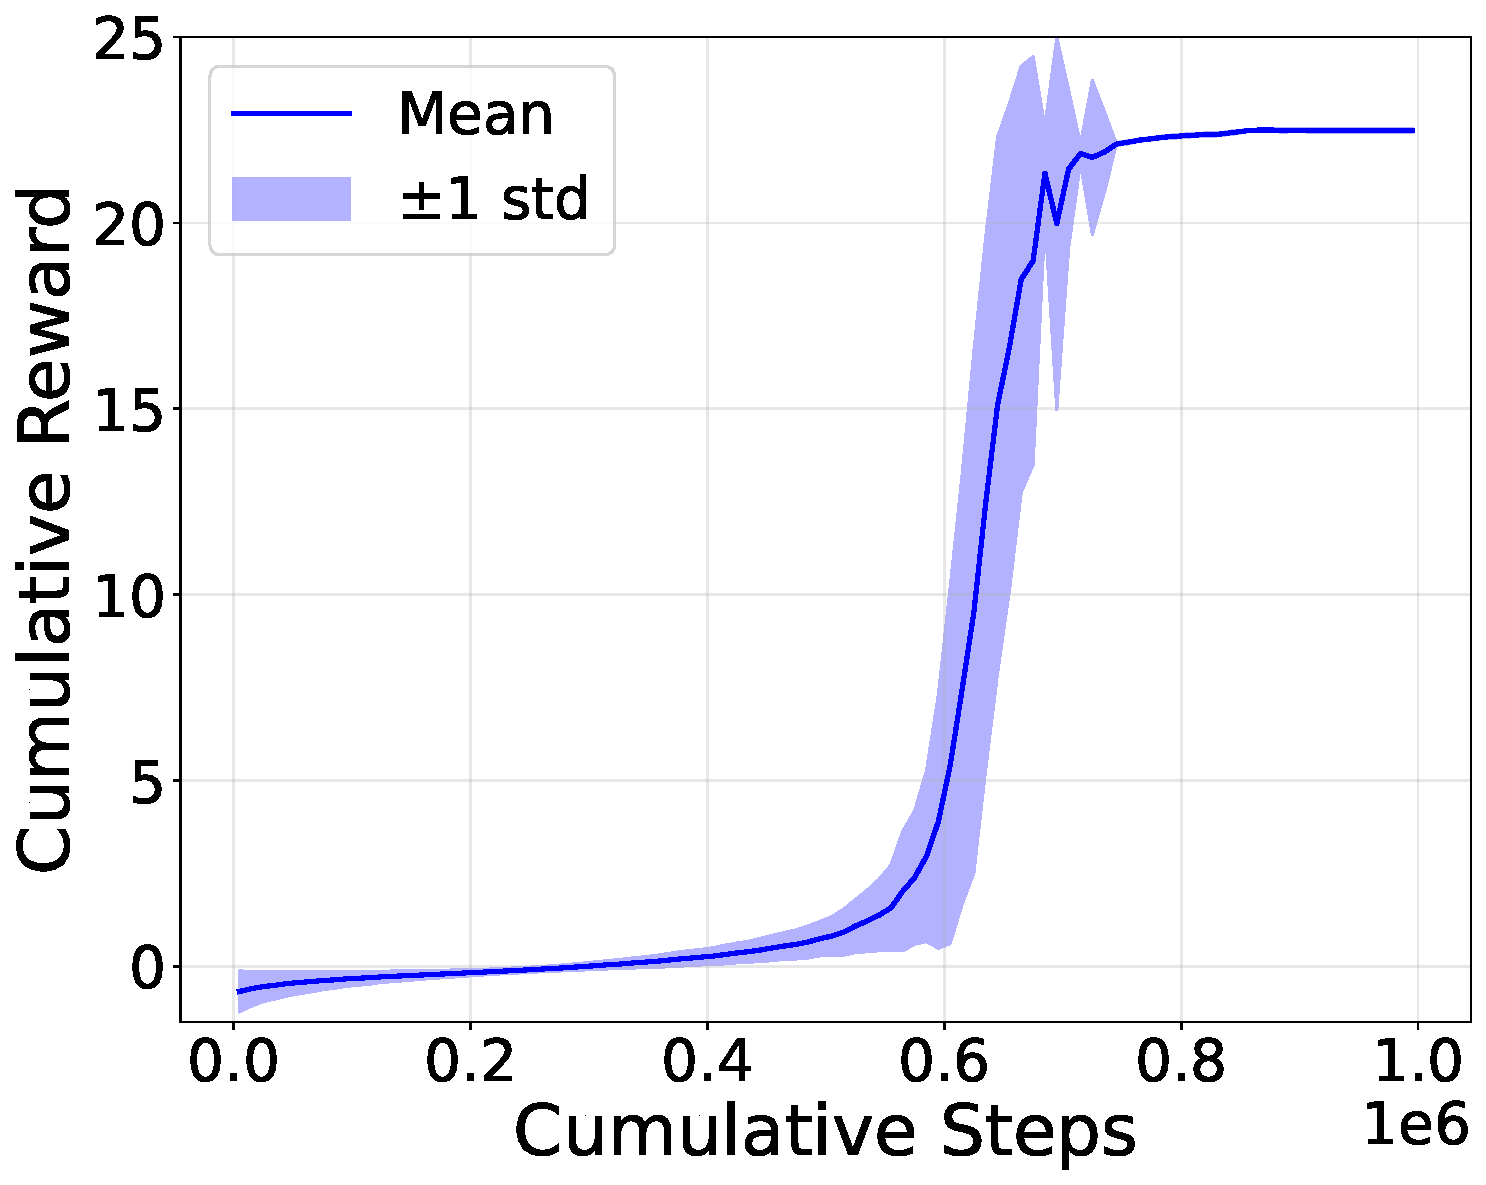
\includegraphics[width=\linewidth]{figs/go1cumulative_reward_readable.pdf}
    \caption{Go1}
    \label{fig:dataset_go1}
  \end{subfigure}
  \hfill
  \begin{subfigure}[t]{0.24\linewidth}
    \centering
    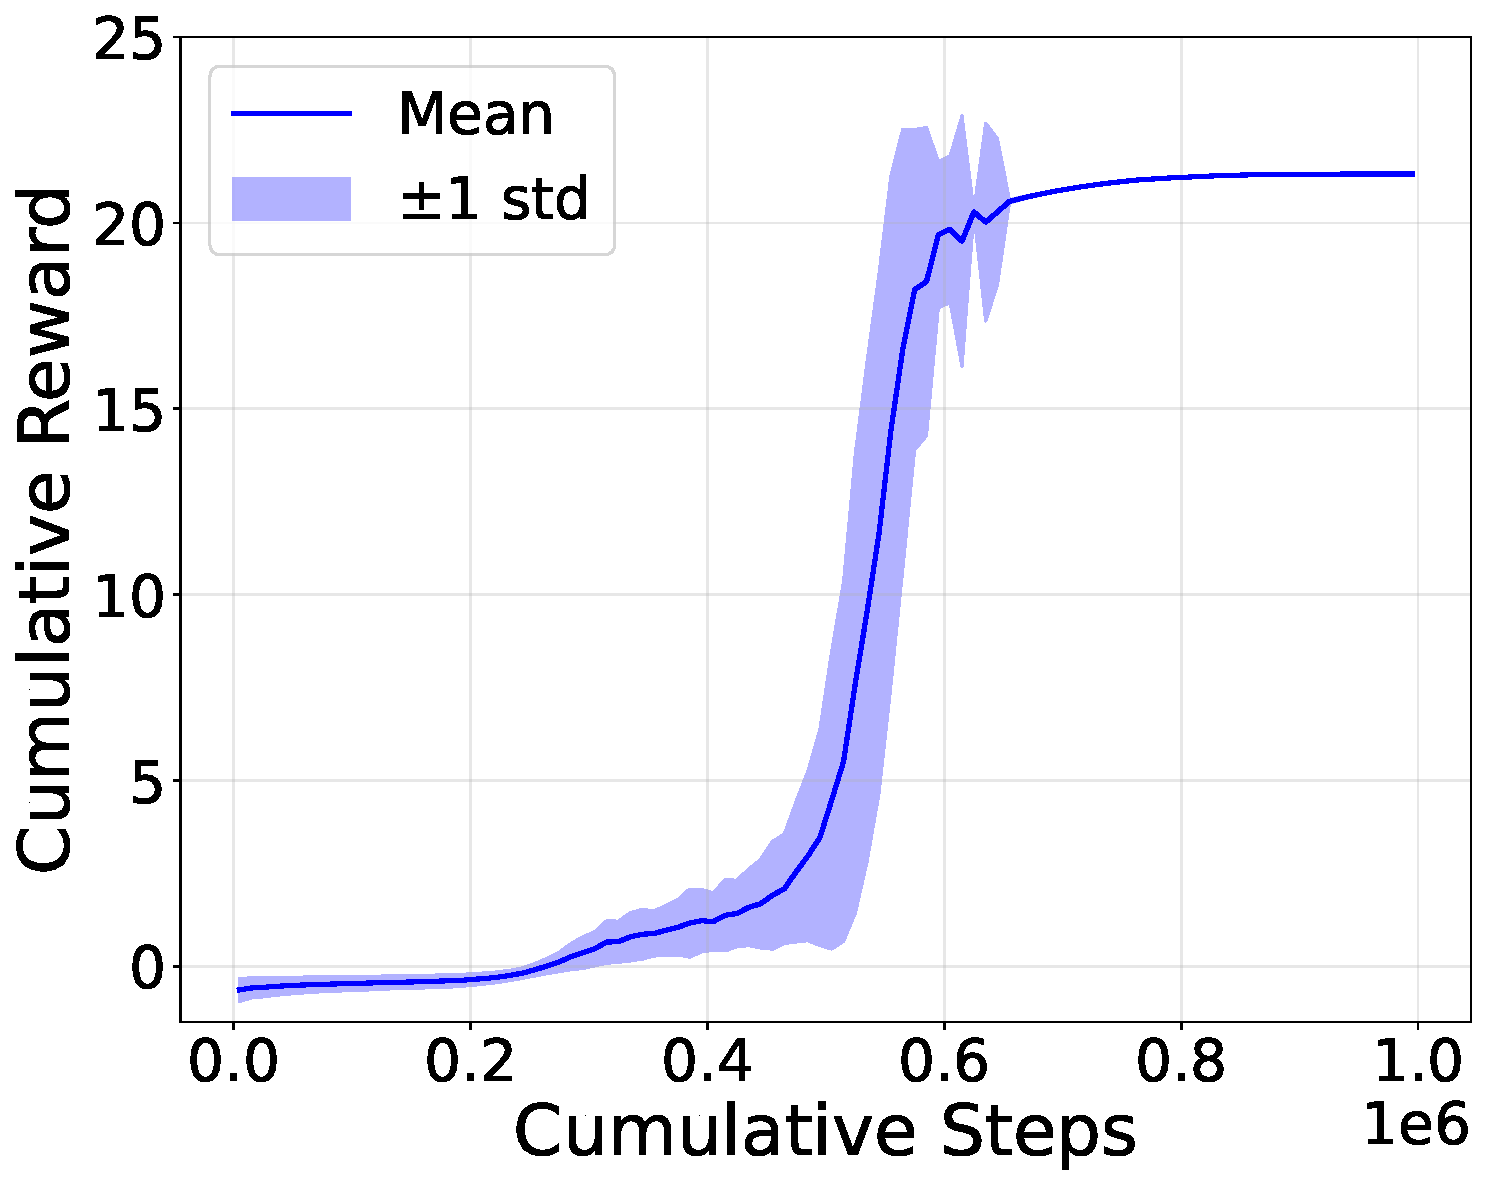
\includegraphics[width=\linewidth]{figs/go2cumulative_reward_readable.pdf}
    \caption{Go2}
    \label{fig:dataset_go2}
  \end{subfigure}
  \hfill
  \begin{subfigure}[t]{0.24\linewidth}
    \centering
    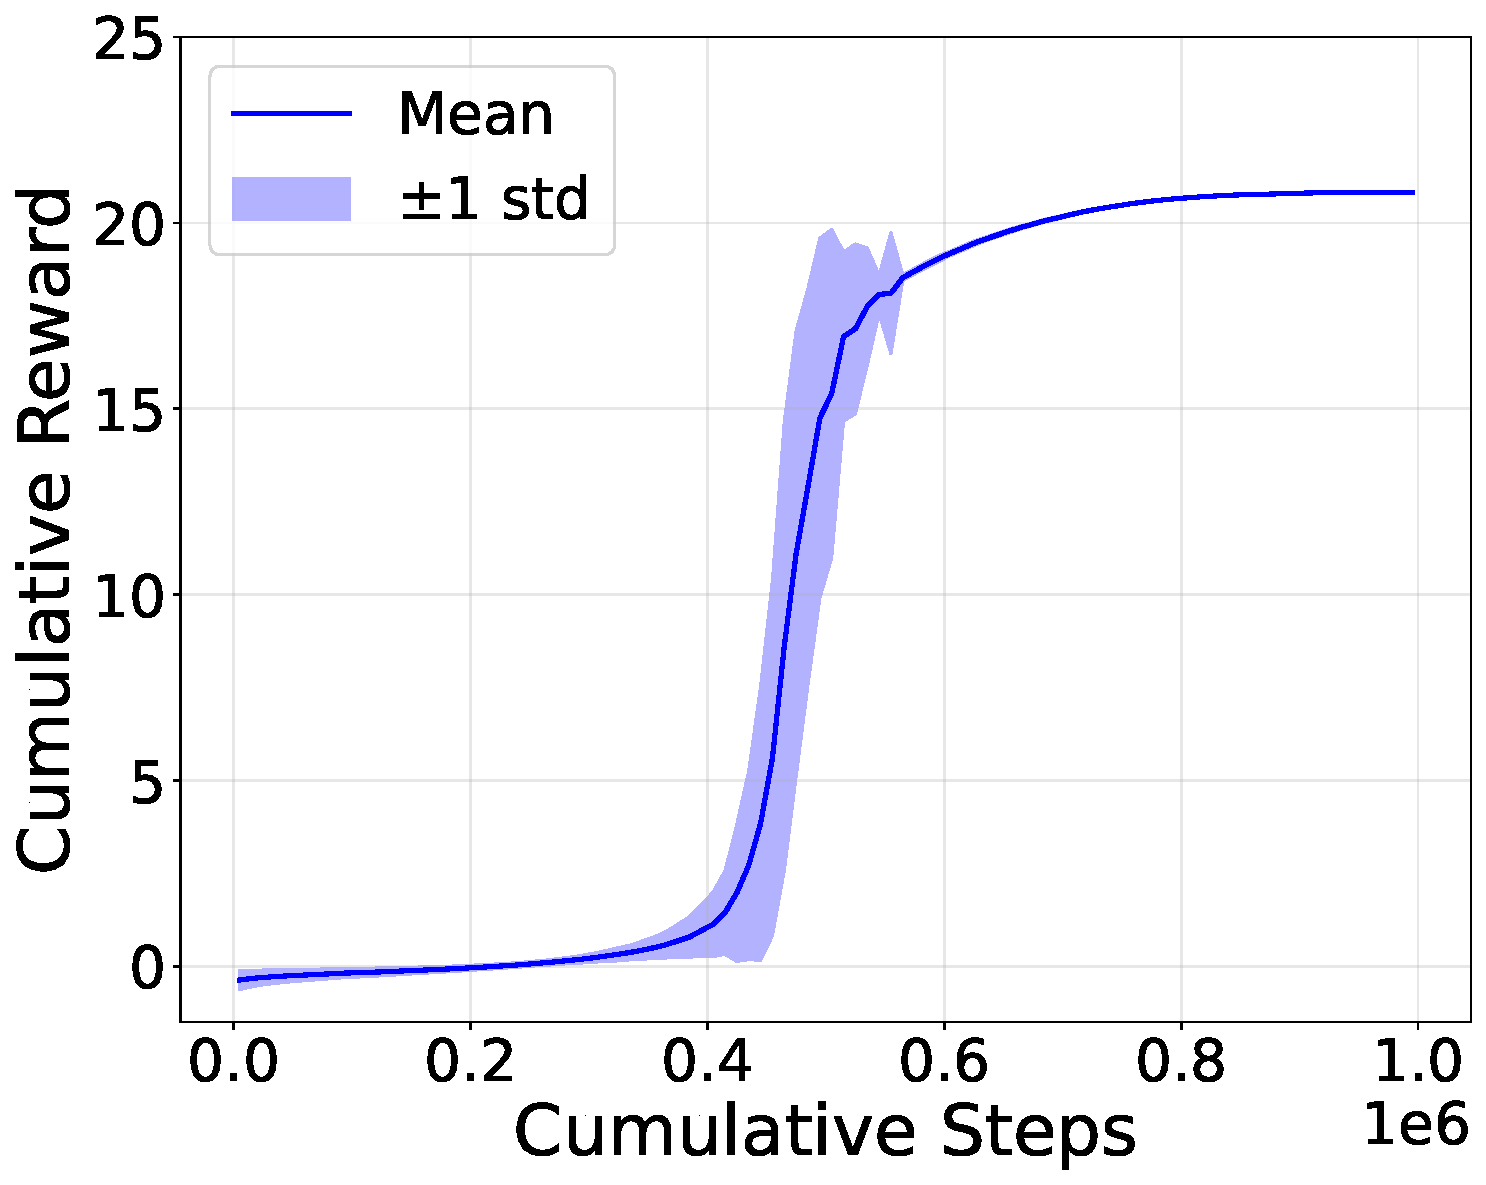
\includegraphics[width=\linewidth]{figs/a1cumulative_reward_readable.pdf}
    \caption{A1}
    \label{fig:dataset_a1}
  \end{subfigure}
  \hfill
  \begin{subfigure}[t]{0.24\linewidth}
    \centering
    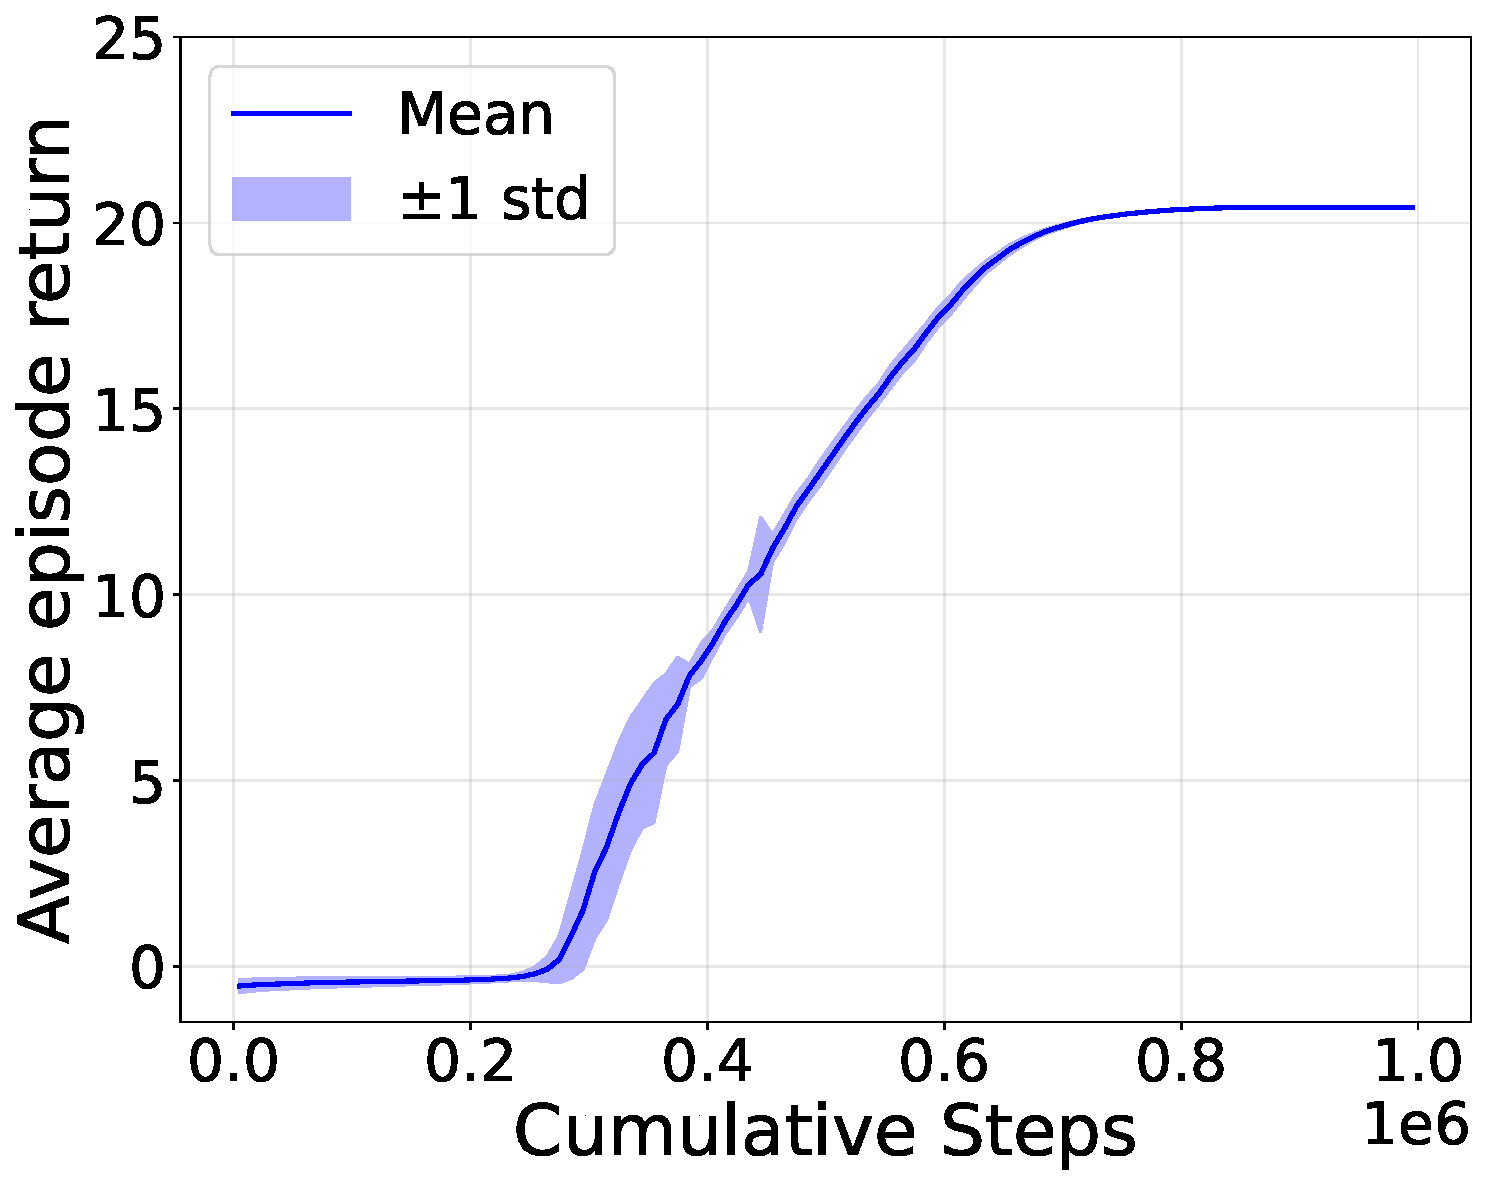
\includegraphics[width=\linewidth]{figs/minicheetahcumulative_reward_readable.pdf}
    \caption{Mini Cheetah}
    \label{fig:dataset_minicheetah}
  \end{subfigure}

  \caption{Average episode return during continuous noise distillation for each robot. As the action noise decreases, the generated behavior gradually approaches that of the corresponding expert policy.}
  \label{fig:dataset_overview}
\end{figure}

\begin{table}[t]
  \centering
  \caption{Physical parameters of the quadrupedal robots.}
  \label{tab:robot_parameters}
    \begin{tabular}{lcccc}
      \hline
      Parameter & Go1 & Go2 & A1 & Mini Cheetah \\
      \hline
      Total mass [kg] & 13 & 15 & 12 & 9 \\
      Body length [m] & 0.38 & 0.38 & 0.27 & 0.28 \\
      Body width [m] & 0.09 & 0.09 & 0.19 & 0.20 \\
      Body height [m] & 0.11 & 0.11 & 0.11 & 0.10 \\
      Thigh link length [m] & 0.21 & 0.21 & 0.20 & 0.21 \\
      Shank link length [m] & 0.21 & 0.21 & 0.20 & 0.21 \\
      \hline
    \end{tabular}
\end{table}

\begin{table}[t]
  \centering
  \caption{Implementation details and hyperparameters. Unless otherwise noted, the settings are shared by all robots.}
  \label{tab:hyperparameters}
  \scriptsize
  \begin{tabular}{@{}p{0.25\linewidth}p{0.71\linewidth}@{}}
    \toprule
    \multicolumn{2}{@{}l}{\textbf{Environment}} \\
    Control & 50~Hz control rate, one-step action latency, maximum episode length of 1000 steps, termination when the roll or pitch angle exceeds $10^\circ$ \\
    Command & Forward velocity 0.5~m/s, lateral velocity 0~m/s, yaw rate 0~rad/s \\
    Observation (33-D) & Base angular velocity ($\times 0.25$), projected gravity, velocity command (scaled by 2.0, 2.0, 0.25), joint-position offsets from the default pose, and joint velocities ($\times 0.05$) \\
    Action (12-D) & Joint-position offsets; target angle $q_{\mathrm{default}} + 0.25\,a_t$, tracked by a PD controller ($K_p = 20$, $K_d = 0.5$) \\
    Reward weights & Linear-velocity tracking 1.0, angular-velocity tracking 0.2 (both $\exp(-e^2/0.25)$), vertical velocity $-1.0$, body height $-50$, action rate $-0.005$, default-pose deviation $-0.1$; each weight is multiplied by the control period (0.02~s) \\
    Target body height & Go1 0.32~m, Go2 0.30~m, A1 0.27~m, Mini Cheetah 0.30~m \\
    \midrule
    \multicolumn{2}{@{}l}{\textbf{Continuous noise distillation}} \\
    Data per robot & Ten trajectories of $N_s = 10^6$ steps each \\
    Schedule & $p = 0.6$, $f = 0.05$; $u_t$ sampled uniformly within the action range given by the joint limits \\
    \midrule
    \multicolumn{2}{@{}l}{\textbf{Model}} \\
    Input embedding & Observation 127-D, action 127-D, reward 2-D (256-D token) \\
    Transformer & 3 layers, 4 heads, hidden size 256, feed-forward size 128, dropout 0.1, LayerNorm, query--key normalization \\
    Decoder & MLP with three hidden layers of 256 units (LeakyReLU) and a 12-D output \\
    \midrule
    \multicolumn{2}{@{}l}{\textbf{Training (pre-training and adaptation)}} \\
    Sequences & Context length 2048, sequence stride 128; observations normalized per robot \\
    Optimization & AdamW, learning rate $3\times10^{-4}$, $(\beta_1, \beta_2) = (0.9, 0.99)$, weight decay 0.1, bf16 \\
    Batch & 8 sequences per mini-batch, gradient accumulation over 8 mini-batches \\
    Epochs & Pre-training 2, adaptation 2 (decoder only) \\
    Seed & 5 \\
    \midrule
    \multicolumn{2}{@{}l}{\textbf{PPO expert (RSL-RL)}} \\
    Network & Actor and critic MLPs with hidden layers (512, 256, 128), ELU, initial action std 1.0 \\
    Optimization & 300 iterations, 24 steps per environment per iteration, 512--4096 parallel environments, 5 epochs, 4 mini-batches, learning rate $10^{-3}$ (adaptive, target KL 0.01), clip 0.2, $\gamma = 0.99$, $\lambda = 0.95$, entropy coefficient 0.01 \\
    \bottomrule
  \end{tabular}
\end{table}

\subsection{Evaluation Protocol}

The target task is quadrupedal locomotion on a planar surface. 
Each episode terminates after 1000 time steps or when the roll or pitch angle of the robot body exceeds 10 degrees. 
The total reward at time step $t$ is the weighted sum of reward and penalty terms:
\begin{equation}
R_{\text{total}}(t) = \sum_{k} w_k R_k(t),
\end{equation}
where $R_k(t)$ and $w_k$ denote the $k$-th reward term and its weight, respectively.

The reward function consists of linear velocity tracking, angular velocity tracking, body height, vertical velocity, action rate, and default-pose deviation terms~\cite{Genesis}. 
The tracking terms encourage the robot to follow the commanded velocity.
The remaining terms promote stable and smooth locomotion.
The weights and the target body heights are listed in Table~\ref{tab:hyperparameters}.

We define the return of an episode of length $T$ as
\begin{equation}
G=\sum_{t=0}^{T-1}R_{\mathrm{total}}(t).
\label{eq:episode_return}
\end{equation}
For each target robot, we run each policy in ten parallel environments, and each environment executes ten consecutive episodes, which yields 100 evaluation episodes per policy.
At the beginning of the evaluation, the base position, the roll and pitch angles, and the joint angles in each environment are perturbed uniformly within $\pm0.1$~m, $\pm5^\circ$, and $\pm0.1$~rad, respectively, without a fixed random seed. The subsequent episodes start from the nominal initial state.
The interaction history is carried across episodes within each environment and is not reset at episode boundaries.
The model conditions on the most recent 2048 transitions, which span approximately two full-length episodes, and the history is initialized only at the beginning of the evaluation.
Therefore, the change in the episode return across successive episodes reflects in-context policy improvement.
We report the mean and standard deviation of the return over the 100 episodes.
The PPO experts are evaluated over 200 episodes (ten environments with 20 episodes each).
All results are obtained from a single pre-training run and a single adaptation run for each target robot (seed 5); results across independent pre-training and adaptation seeds are not available.

We compare the following three policies:
\begin{itemize}
  \item \textbf{Zero-shot Algorithm Distillation:}
  the pretrained model is applied to the held-out robot without parameter updates;
  \item \textbf{Decoder-only adaptation:}
  the proposed method fine-tunes only the decoder using 10\% of the target-robot data;
  \item \textbf{PPO expert:}
  a robot-specific expert policy is trained directly on the target robot.
\end{itemize}
We use RSL-RL~\cite{schwarke2025rslrllearninglibraryrobotics} to train the PPO expert policies.



\FloatBarrier  % Float Boundary


\subsection{Results}

\begin{table}[H]
\centering
\caption{Episode return on each held-out target robot (mean $\pm$ standard deviation over the evaluation episodes).
    The expert ratio is the mean return of the decoder-adapted policy divided by that of the corresponding PPO expert.}
\label{tab:adaptation_results_inv}
\begin{tabular}{lcccc}
\toprule
\textbf{Method} & \textbf{Go1} & \textbf{Go2} & \textbf{A1} & \textbf{Mini Cheetah} \\
\midrule
Zero-shot Algorithm Distillation & $15.17 \pm 1.07$ & $0.53 \pm 0.13$ & $15.19 \pm 7.70$ & $-0.17 \pm 0.04$ \\
 Decoder-only adaptation (ours) & $19.3 \pm 7.4$ & $21.2 \pm 0.1$ & $20.7 \pm 0.1$ & $20.0 \pm 2.0$ \\
 PPO expert & $22.5 \pm 0.03$ & $21.3 \pm 0.01$ & $20.9 \pm 0.02$ & $21.1 \pm 0.03$ \\
\midrule
Expert ratio [\%] & 85.7 & 99.6 & 99.2 & 94.9 \\
\bottomrule
\end{tabular}
\end{table}

\begin{figure}[t]
  \centering
  \captionsetup[subfigure]{font=tiny}

  \begin{subfigure}[t]{0.24\linewidth}
    \centering
    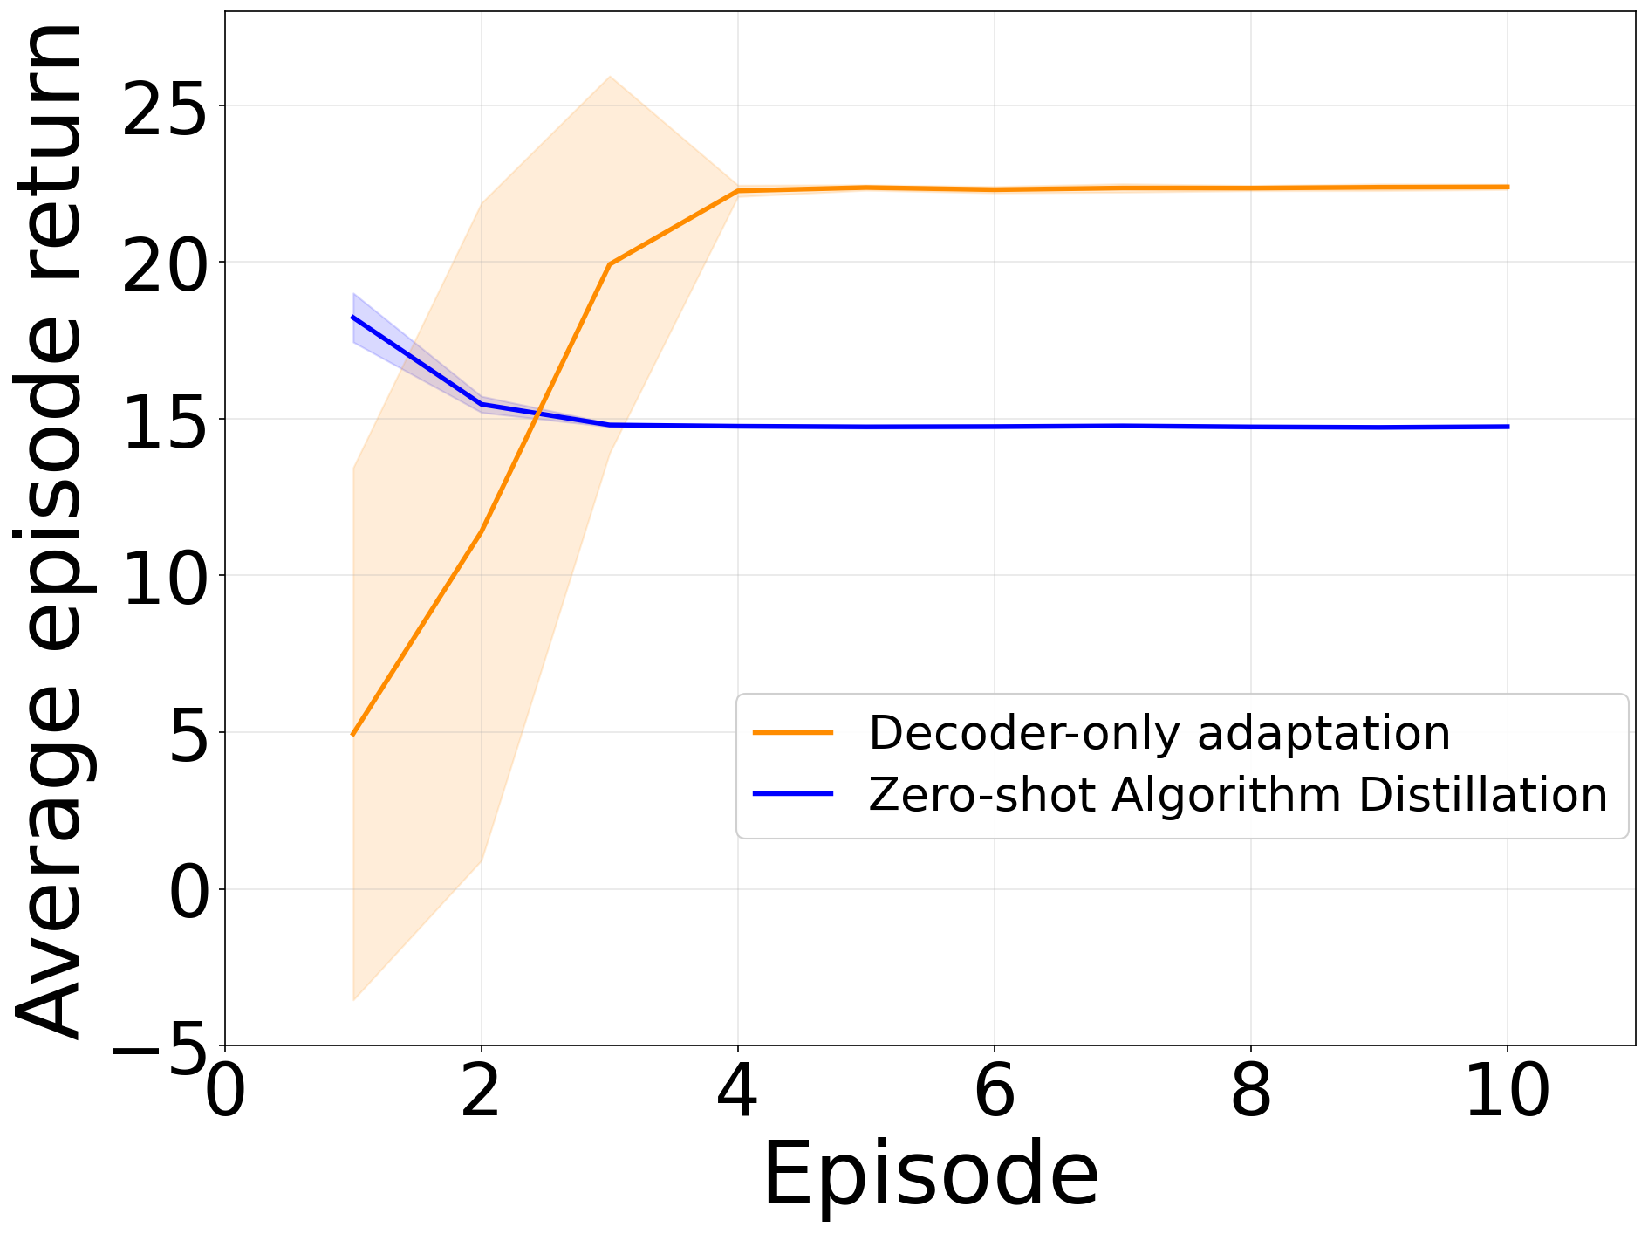
\includegraphics[width=\linewidth]{figs/go1_without_vs_finetune_final.pdf}
    \caption{Go1}
  \end{subfigure}
  \hfill
  \begin{subfigure}[t]{0.24\linewidth}
    \centering
    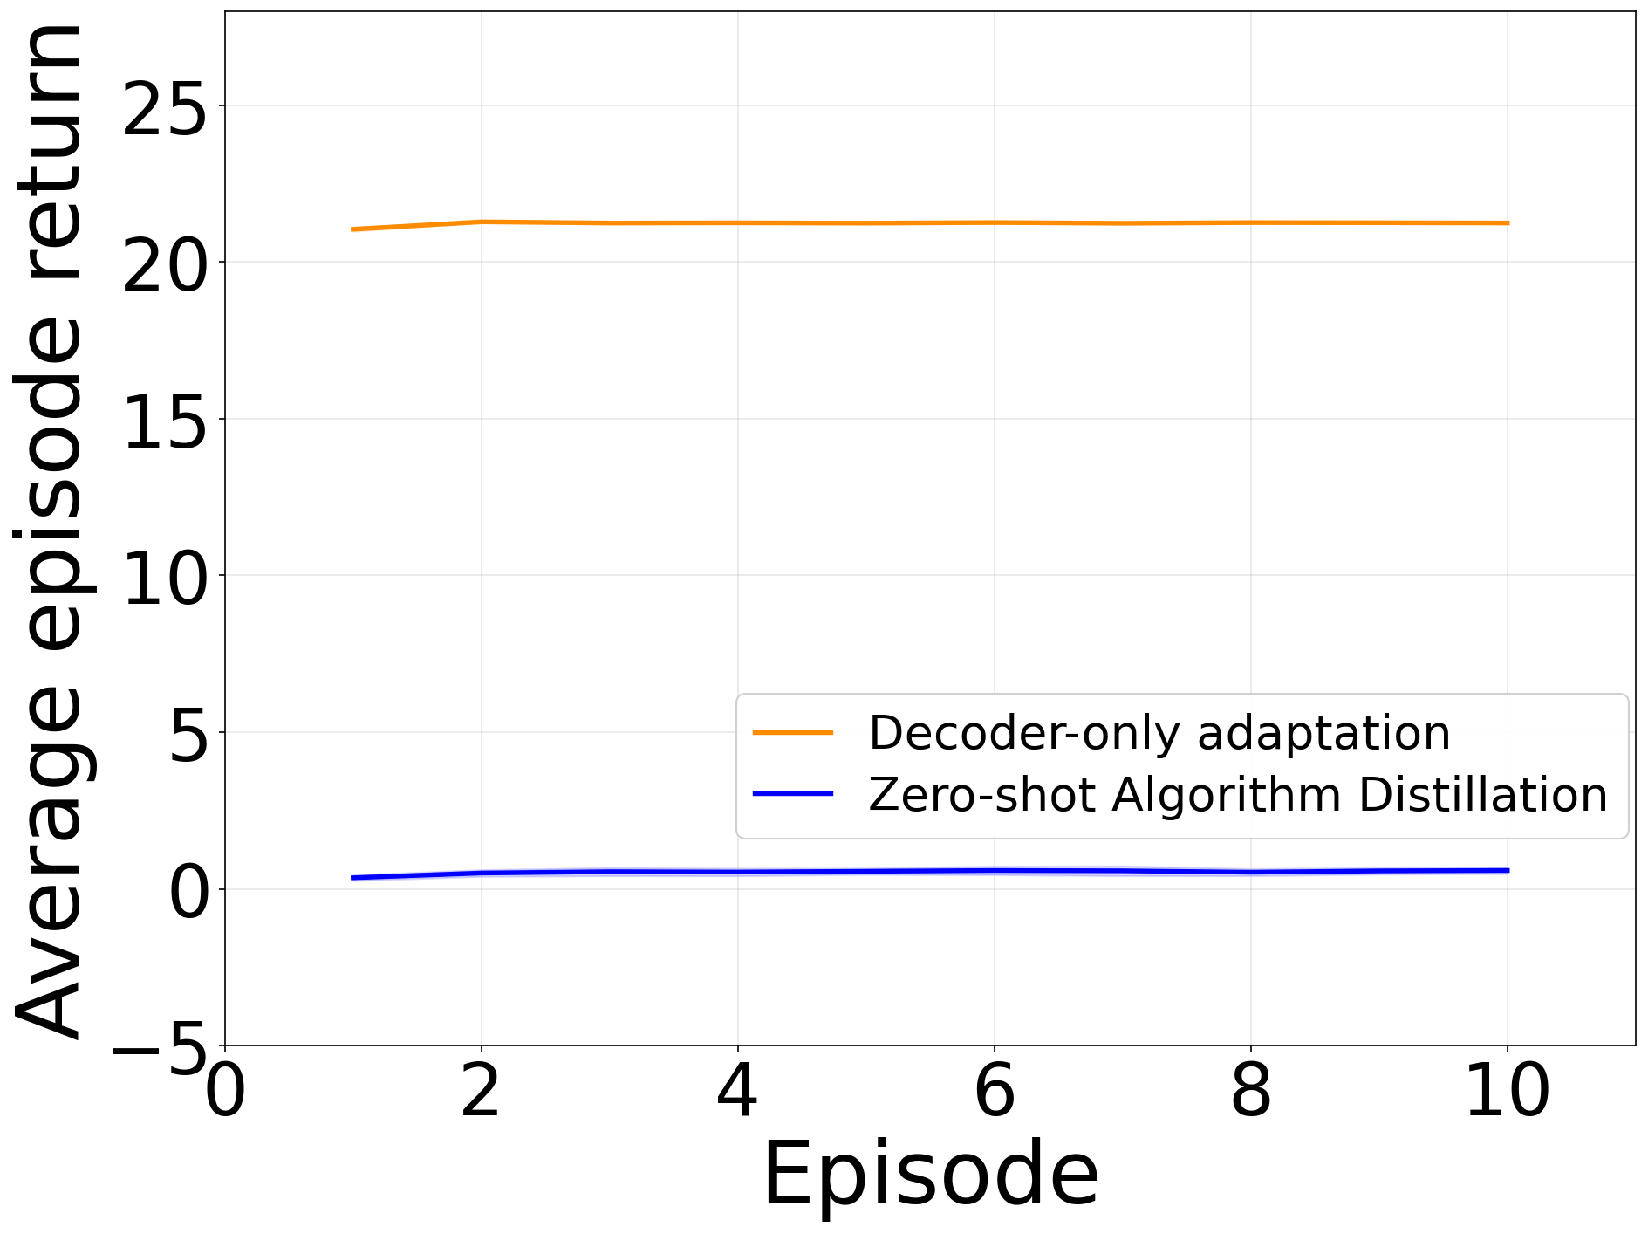
\includegraphics[width=\linewidth]{figs/go2_without_vs_finetune_final.pdf}
    \caption{Go2}
  \end{subfigure}
  \hfill
  \begin{subfigure}[t]{0.24\linewidth}
    \centering
    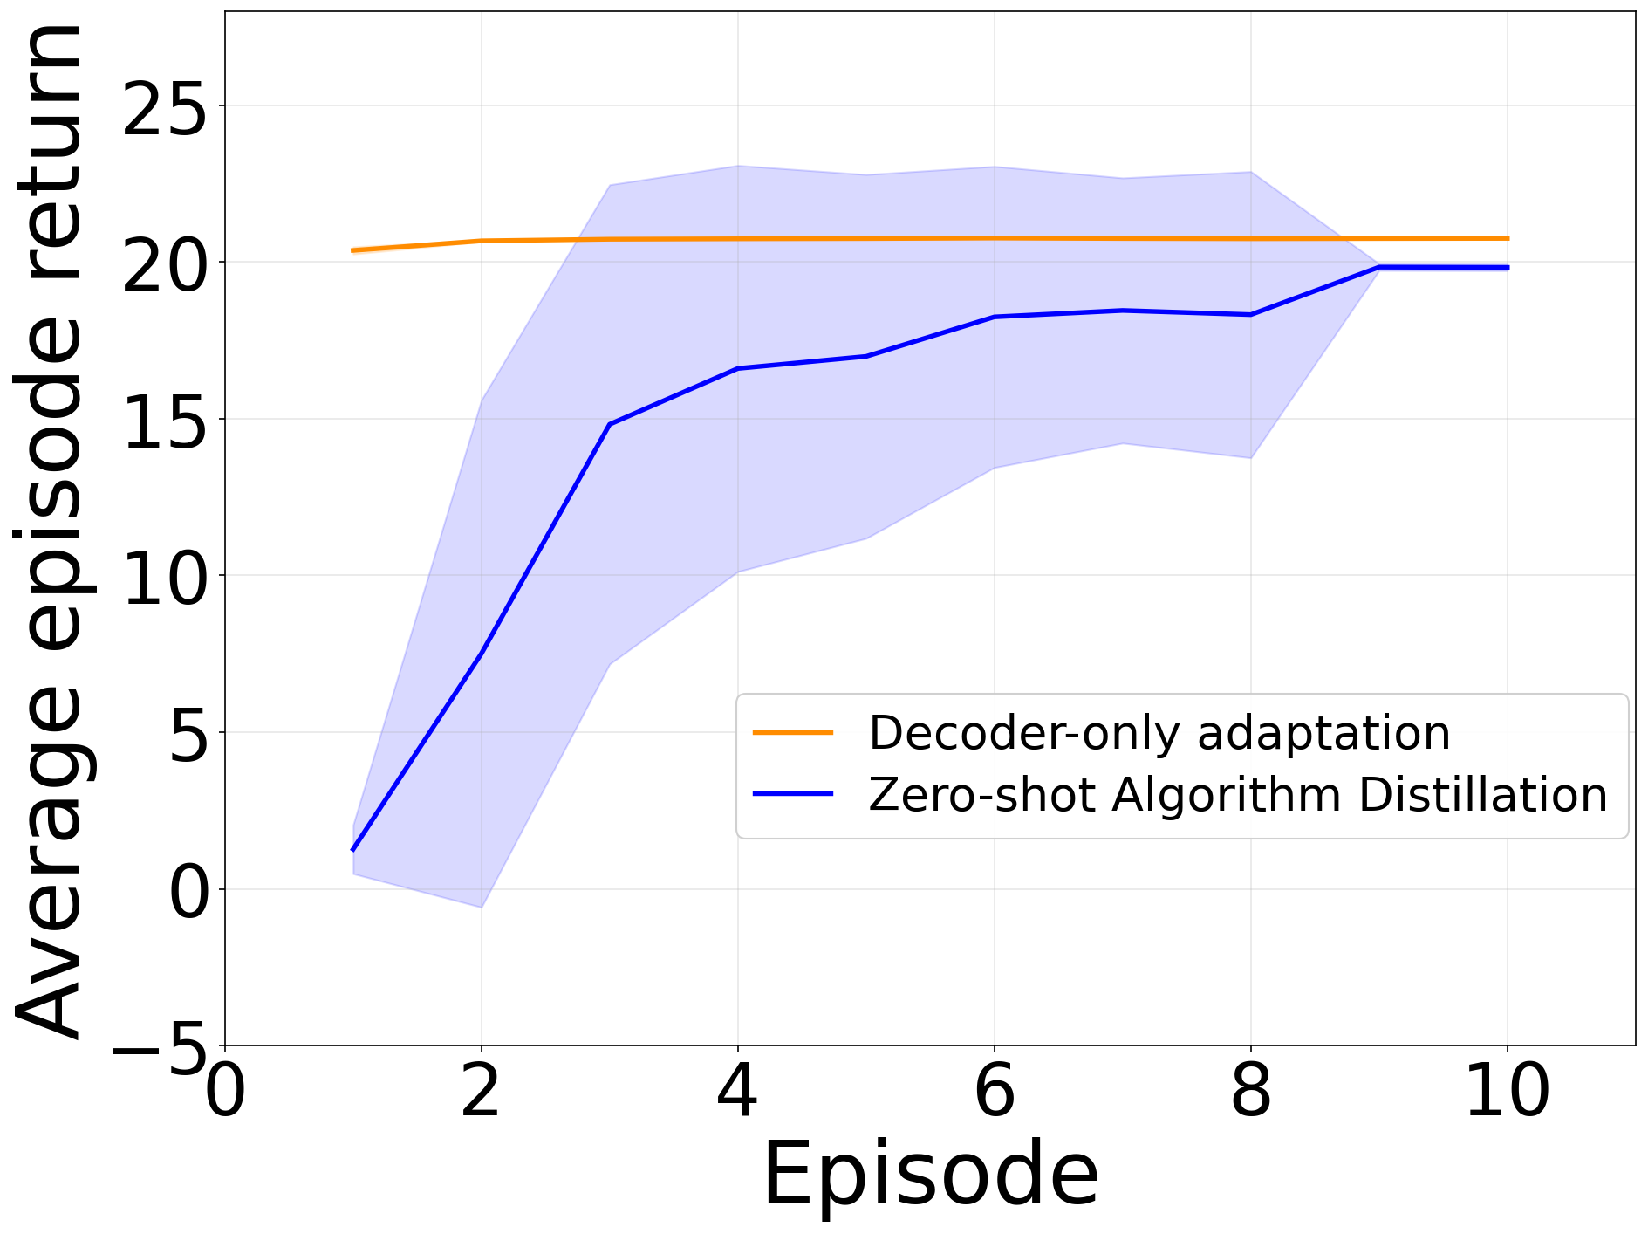
\includegraphics[width=\linewidth]{figs/a1_without_vs_finetune_final.pdf}
    \caption{A1}
  \end{subfigure}
  \hfill
  \begin{subfigure}[t]{0.24\linewidth}
    \centering
    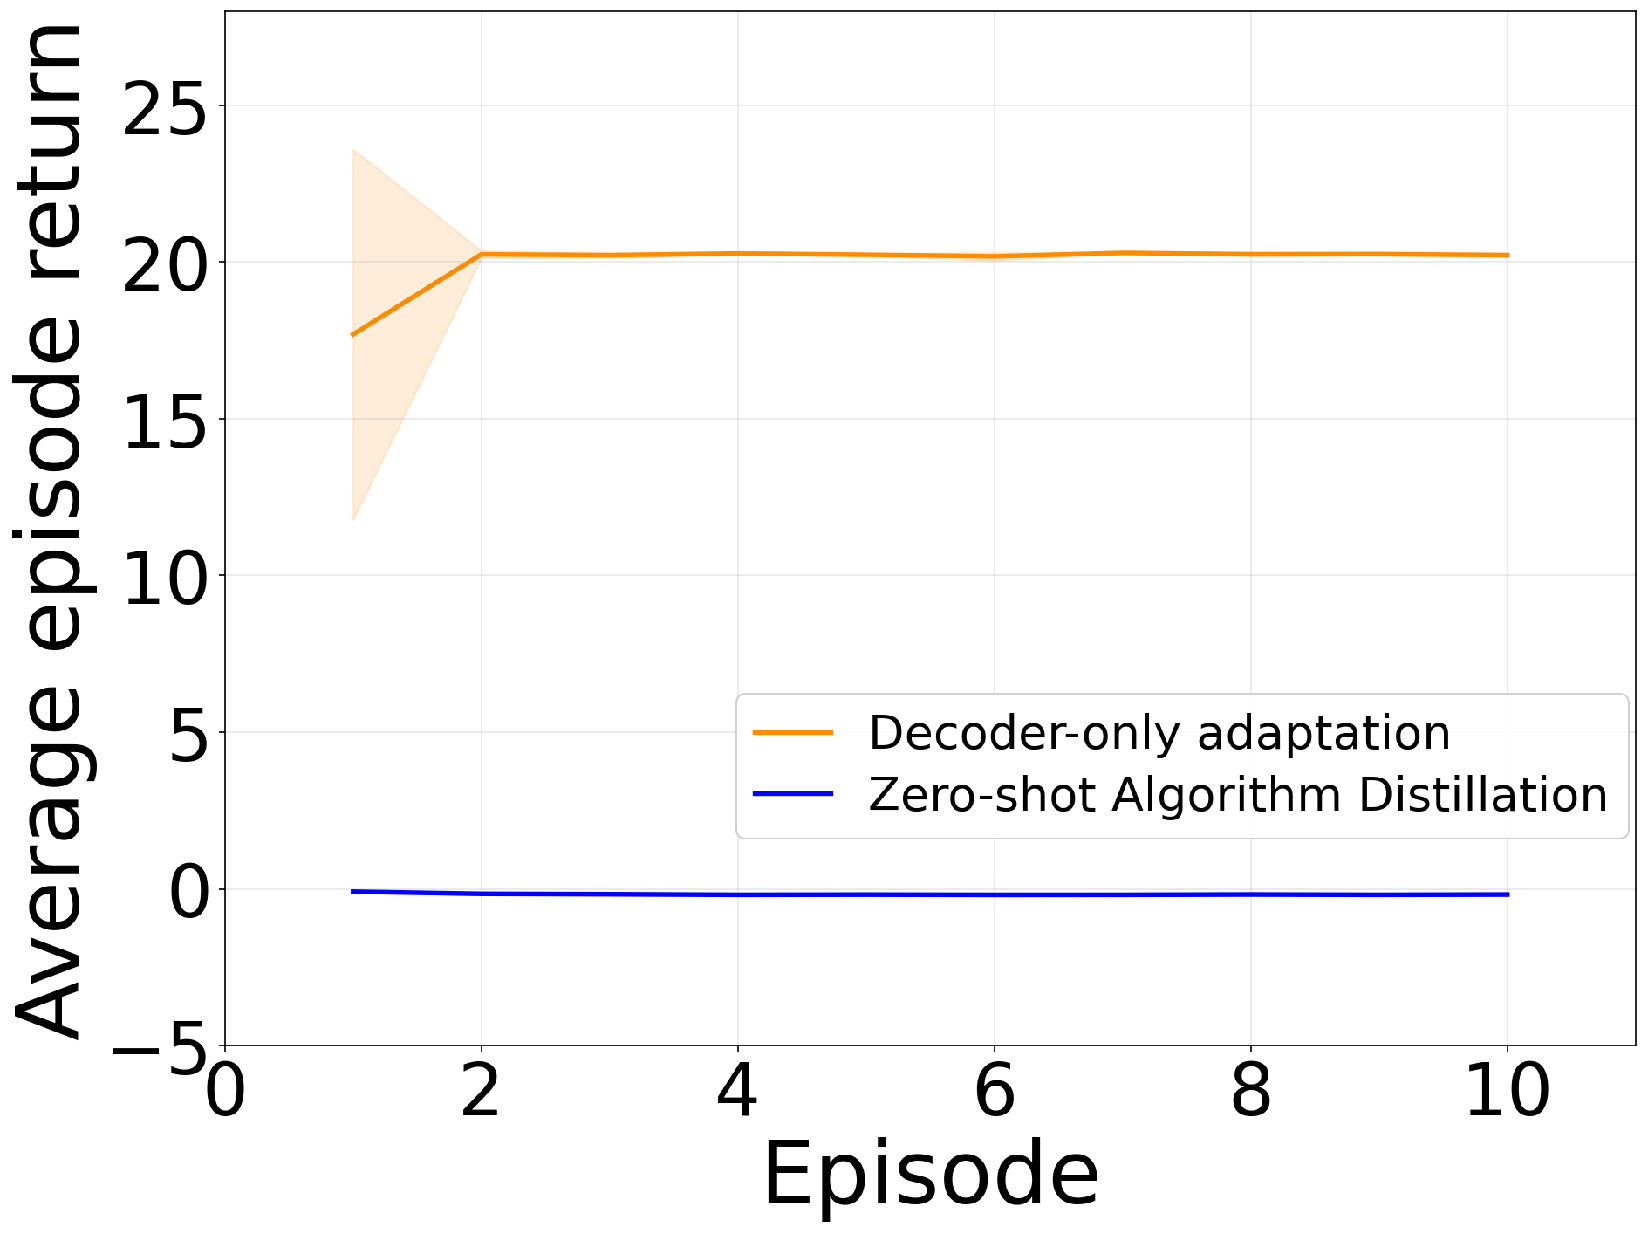
\includegraphics[width=\linewidth]{figs/minicheetah_without_vs_finetune_final.pdf}
    \caption{Mini Cheetah}
  \end{subfigure}

  \caption{Episode return curves before (Zero-shot) and after (Decoder-only adaptation) on the held-out target robots. Each environment executes ten consecutive episodes while the interaction history is carried across episodes. The curves show the return of the $k$-th episode averaged over the ten environments, and the shaded regions indicate one standard deviation across the environments.}
  \label{fig:adaptation}
\end{figure}

Table~\ref{tab:adaptation_results_inv} summarizes the average episode return on each held-out target robot. 
The zero-shot algorithm-distilled policy achieves returns of 15.17, 0.53, 15.19, and $-0.17$ on Go1, Go2, A1, and Mini Cheetah, respectively.
Thus, zero-shot transfer performs reasonably well on Go1 and A1 but performs poorly on Go2 and Mini Cheetah.
Decoder-only adaptation (ours) yields a higher average episode return than the zero-shot policy for all four robots.
The adapted policies achieve returns of 19.3, 21.2, 20.7, and 20.0 for Go1, Go2, A1, and Mini Cheetah, respectively. These values correspond to 85.7\%, 99.6\%, 99.2\%, and 94.9\% of the returns achieved by the corresponding expert policies.

The largest increases are observed on Go2 and Mini Cheetah, for which
decoder-only adaptation increases the average return by 20.70 and
20.16, respectively.
The increases on Go1 and A1 are 4.10 and 5.52, respectively.
Thus, the improvement is particularly large for the two robots on which
the zero-shot policy achieves returns close to zero.


Figure~\ref{fig:adaptation} shows the episode returns before and after decoder-only adaptation.
Under zero-shot transfer, the returns for Go2 and Mini Cheetah remain
close to zero, while the return for A1 increases over successive
episodes.
After decoder-only adaptation, the return for Go1 increases during the first three episodes and then stabilizes.
Mini Cheetah shows a lower return with a large variation only in the first episode,
whereas Go2 and A1 maintain high returns from the first episode.
The shaded regions indicate one standard deviation of the $k$-th episode return across the ten environments.

The standard deviation in Table~\ref{tab:adaptation_results_inv} is large for the adapted policy on Go1 ($\pm7.4$).
This dispersion originates from the first three episodes, in which eight, five, and one of the ten environments terminate early, respectively, before the in-context improvement takes effect.
From the fourth to the tenth episode, the adapted policy on Go1 achieves $22.35 \pm 0.12$.
The dispersion on Mini Cheetah ($\pm2.0$) is caused by a single early termination in the first episode, and the return from the second to the tenth episode is $20.24 \pm 0.09$.
The adapted policies on Go2 and A1 achieve stable returns from the first episode ($\pm0.1$ on both robots).



\subsection{Discussion}
The zero-shot results vary substantially across the held-out target robots.
The pretrained policy transfers relatively well to Go1 and A1 but achieves returns close to zero on Go2 and Mini Cheetah.
This variation suggests that the interaction history alone does not always compensate for physical differences that are absent from the pre-training data.

Decoder-only adaptation yields higher average episode returns for all four robots, with particularly large increases on Go2 and Mini Cheetah.
The adapted policies reach 85.7--99.6\% of the returns achieved by the corresponding PPO experts.
These results demonstrate the benefit of decoder adaptation and are consistent with our hypothesis that the pretrained history encoder retains locomotion features that remain useful across robots, while the decoder adjusts the output mapping to the target robot.
However, the present results do not isolate the contribution of the encoder.
We do not compare decoder-only adaptation with full-model fine-tuning, with a newly initialized decoder trained on the fixed encoder, or with training from scratch using the same amount of target data.
Without such matched-data comparisons, the improvement cannot be attributed to the transferability of the history encoder, and the results do not establish that transferable locomotion information is contained in the encoder or that robot-specific differences are confined to the decoder.

The adaptation data are generated from a PPO expert trained on the target robot.
Therefore, the present experiments evaluate parameter-efficient adaptation from target-robot expert demonstrations rather than parameter-free adaptation to a new robot.
When discussing practical efficiency, the cost of decoder fine-tuning should be distinguished from the cost of preparing the adaptation data.
Decoder fine-tuning updates 16.3\% of the model parameters with 242 parameter updates and takes approximately two minutes on a single GPU.
In contrast, the target-specific PPO expert is trained for 300 iterations with 512--4096 parallel environments, which corresponds to $3.7\times10^6$--$2.9\times10^7$ environment steps and 6,000 gradient updates, and continuous noise distillation requires an additional $10^7$ environment steps.
Thus, the present method does not reduce the cost of obtaining a target-robot expert; its efficiency lies in adapting the pretrained model to the target robot with a small number of parameter updates.

Deploying the method on real hardware involves one assumption and one main challenge.
The method assumes that a simulation model of the target robot is available.
The adaptation data are generated by applying continuous noise distillation to a target-robot PPO expert, and even the 10\% adaptation set covers approximately $8\times10^6$ distinct transitions; executing such strongly perturbed actions on a physical robot would risk falls and hardware damage.
Therefore, the adaptation is performed in simulation, and the adapted policy is then transferred to the physical robot.
The policy observations consist only of proprioceptive quantities that are available on physical robots: the base angular velocity, the projected gravity, the velocity command, and the joint positions and velocities.
The rewards in the interaction history additionally depend on the base linear velocity and the body height, which are obtained from the simulator in our experiments and can be supplied by an onboard state estimator on hardware.
The main challenge is robustness to the gap between simulation and hardware.
The expert policies and datasets are generated without randomizing physical parameters, sensor noise, or external disturbances, and the evaluation is limited to flat terrain and a constant forward-velocity command.
Consequently, the adapted policy may be sensitive to discrepancies in actuator dynamics and contact, and to noise in the observations and in the rewards computed from estimated quantities.
This challenge can be addressed by applying domain randomization~\cite{8202133,8460528} to physical parameters, sensor noise, and external disturbances when training the experts and generating the pretraining and adaptation datasets, so that the interaction histories cover these variations.
With this extension, adaptation in simulation can be combined with established sim-to-real techniques to deploy the adapted policy on physical robots.


\section{Conclusion}
\label{conclusion}
This study investigates cross-robot adaptation of an algorithm-distilled locomotion policy. 
The model is pretrained on multiple quadruped robots, and only its decoder is fine-tuned for a robot excluded from pre-training.
In leave-one-robot-out experiments, the adapted policies achieve 85.7--99.6\% of the returns obtained by the corresponding PPO experts.
These results show that adaptation across robot embodiments can be achieved while limiting parameter updates to the output mapping.
They are consistent with the hypothesis that the pretrained history representation is reusable across robots; however, attributing the improvement to the encoder requires matched-data comparisons with full-model fine-tuning and a newly initialized decoder.
This finding contributes to the study of reusable control representations and suggests a possible route toward reducing the number of parameter updates required when deploying controllers on diverse quadruped platforms.

The present study is limited to four simulated robots with similar kinematic structures and relies on expert demonstrations from each target robot.
Future work will examine adaptation from non-expert interaction data, compare decoder-only adaptation with full-model fine-tuning, a newly initialized decoder, and training from scratch under matched target data, report results across multiple pre-training and adaptation seeds, evaluate robots with larger morphological and dynamic differences, and validate the method on real hardware.


\section*{Acknowledgements}

This work was supported by JSPS KAKENHI Grant Numbers JP23K24914 and JP26K02967.

\bibliographystyle{splncs04}
\bibliography{refs}


%\end{thebibliography}
\end{document}